\documentclass[conference]{IEEEtran}
\usepackage{times}

% numbers option provides compact numerical references in the text. 
\usepackage[numbers]{natbib}
\usepackage{multicol}
\usepackage[bookmarks=true]{hyperref}
\usepackage{graphicx}
\usepackage{amsmath,amsfonts,amssymb}
\usepackage{hyperref}
\usepackage{algpseudocode}

\graphicspath{ {./graphics/} }

\pdfinfo{
   /Author (Mingyo Seo)
   /Title  (Robots: Our new overlords)
   /CreationDate (D:20101201120000)
   /Subject (Robots)
   /Keywords (Robots;Overlords)
}

\begin{document}

% paper title
\title{CS391L HW5: Reinforcement Learning}

% You will get a Paper-ID when submitting a pdf file to the conference system
\author{Mingyo Seo}

\author{\authorblockN{Mingyo Seo}
\authorblockA{
UT EID: ms84662\\
Email: mingyo@utexas.edu}}



\maketitle

\IEEEpeerreviewmaketitle

\begin{abstract}

In this assignment, an overview of Q learning is presented and is applied to episodes where an agent walks while picking up litter and avoiding obstacles.
I build a reinforcement learning environment of 4 different tasks.
These tasks were separated for training the corresponding modules independently, and the individual Q matrices were obtained by combining the trained module as a simple weighted sum. 
The state-space search for the Q learning problem was simplified by limiting search grids nearby the agent.
As a result of training, the agent was able to successfully perform tasks in randomly generated environments.
\end{abstract}

\section{Introduction} % Introduce your problem and the overall plan for approaching your problem

In this assignment, we train an agent for the following tasks: 1. picking up litter, 2. avoiding obstacles, 3. staying on the sidewalk, and 4. walking forward.
In each episode, an environment is given with obstacles, litter, and the sidewalk. 
Each environment is defined as a $6 \times 25$ grid where the middle 4 columns as the sidewalk.
Litter and obstacles are randomly scattered along with these grid points.
Therefore, each gridpoint has 3 states as {\it litter}, {\it obstacle} or {\it empty}.
The agent can move to adjacent grids every step.
In addition, we do not consider the agent's action that does not do anything, which results in no change in the environment or the agent.


The answers to the HW5 questions are included in the following sections.
\begin{itemize}
\item Fig. \ref{fig:forward}, \ref{fig:forward_eval}: Training and evaluation of the forward module
\item Fig. \ref{fig:sidewalk}, \ref{fig:sidewalk_eval}: Training and evaluation of the sidewalk module
\item Fig. \ref{fig:litter}, \ref{fig:litter_eval}: Training and evaluation of the litter module
\item Fig. \ref{fig:obstacle}, \ref{fig:obstacle_eval}: Training and evaluation of the obstacle module 
\item Fig. \ref{fig:safe}, \ref{fig:greedy}: Evaluation of the final module
\end{itemize}

\section{Method}
\label{sec:method}

\subsection{RL environment definition}
To train the agent by reinforcement learning, during training episodes, the agent receives an incentive for picking up litter and penalty for encountering obstacles.
Also, training episodes are terminated if the agent reach either the end of the environment.
Optimizing the agent's policy with a full state model of the environment requires a large state space to search.
Each grid has three sates of {\it litter}, {\it obstacle}, and {\it empty}, so the size of the state space can be computed as,
\begin{equation}
\begin{aligned}
(6 \times 25) \times 4^{6\times25}  \approx  3.1 \times 10 ^{92}
\end{aligned}
\end{equation}
Due to the large scale of the state space, we consider the following 2 methods to reduce the problem size: 1. training an independent module for each task, and 2. limiting the range of grids nearby the agent that the agent search.

\subsection{$\epsilon$-greedy algorithm}
The $\epsilon$-greedy algorithm is a probabilistic decision-making algorithm. 
It allows us to control the agent's tendency of exploration and exploitation by varying the $\epsilon$ value.
Given 3 or more different possible actions, the epsilon greedy algorithm can be implemented as:

\begin{algorithmic}
\State $\theta$ is sampled from the uniform distribution $U(0,1)$
\If{$\theta < \epsilon$} 
    \State Choose a random action
\ElsIf{$\theta \leq \epsilon$}
	\State Choose the action $a^*=\operatorname*{argmax}_a Q(s,a)$
\EndIf 
\end{algorithmic}
Here, high values can cause instability in training.

\subsection{Q learning algorithm}
In this assignment, the Q learning algorithm is used to deal with finite state and action spaces.
Each value at the Q table is initialized to initial values and is updated with collected data of the
corresponding state-action pairs using the following formulation:
\begin{equation}
\begin{aligned}
\label{eq:q}
Q(s, a) \leftarrow (1 - \alpha) Q(s, a) + \alpha \left(R(s, a) + \gamma \max_{a\sp{\prime}}
Q(s\sp{\prime}, a\sp{\prime})
\right).
\end{aligned}
\end{equation}
Here $s$, $a$ are the current state and action respectively, $s\sp{\prime}$ is
the state acquired after by taking action $a$ in state $s$, and $\alpha$, $\gamma$ are hyperparameters that determine the rate of learning and the emphasis on future rewards respectively.
Then, all the rows of the Q table are normalized using the L1 norm for each row. 
The final policy used by the agent is the policy of maximizing Q as,
\begin{equation}
\begin{aligned}
a^{*} = \Pi (s)=\max_{a} Q(s, a).
\end{aligned}
\end{equation}

\subsection{Weighted sum for action selection}
The normalized Q tables of the 4 different tasks were combined using a simple weighted sum.
Let $Q_i$ and $w_i$ be the Q table and the weight of the $i$ task module.
Then, the states $s_i$ for the modules are determined at each step.
For each action $a$, the Q weighted values were generated as,
\begin{equation}
\begin{aligned}
Q_{final}(s, a) = \sum_{i} w_i Q_i(s_i, a).
\end{aligned}
\end{equation}
The final policy is to choose the action that maximizes the weighted Q value as,
\begin{equation}
\begin{aligned}
a^{*} = \max_{a} Q_{final}(s, a).
\end{aligned}
\end{equation}

\section{Modules}
\label{sec:method}

\subsection{Forward module}
The forward module takes the position component and dimensions of the full state.
To train the agent to walk forward, we give an incentive for reaching the end of the grid, which is defined as a terminal state.
Otherwise, the agent does not receive any incentive.
In this assignment, we used a binary reward design where a reward is 1 at the terminal state and 0 otherwise.

\subsection{Sidewalk module}
The sidewalk module also takes the position component and dimensions of the full state.
To train the agent to stay on the sidewalk, we give a penalty for staying out of the sidewalk grids.
Otherwise, the agent does not receive any penalty.
In this assignment, we used a binary reward design where a reward is -1 outside the sidewalk and 0 otherwise.

\subsection{Litter module}
The litter module assumes the limited search grid range of the agent.
It takes the $5 \times 5$ position component and binary states of {\it litter} and {\it empty}, and the agent is assumed to be in the middle grid position.
Actions in the module are the same as the original state space where they shift the grid $5 \times 5$ to locate the agent in the middle of the grid.
As with the original, litter is collected when the agent moves to a position with litter and the state at the grid changed from {\it litter} to {\it empty}.
To encourage the agent to collect litter, we give an incentive for reaching grids where litter is located.
For this assignment, we used a binary reward design where a reward is 1 at {\it litter} grid and 0 otherwise.
Once the agent collects all the litter, the grid is reinitialized with random litter.
In addition, to reduce the gap between the training environments of reduced grids and the test environments of full grids, we used the same probability of litter on the grids.

\subsection{Obstacle module}
The Obstacle module also assumes the limited search grid range of the agent.
Likewise, it takes the $5 \times 5$ position component and binary states of {\it obstacle} and {\it empty}, and the agent is assumed to be in the middle grid position.
Actions work as same as the litter module.
To discourage the agent to encounter an obstacle, we give a penalty for reaching grids where an obstacle is located.
For this assignment, we used a binary reward design where a reward is -1 at {\it obstacle} grid and 0 otherwise.
Also, to reduce the gap between the training environments of reduced grids and the test environments of full grids, we used the same probability of obstacles on the grids.

\section{Results} % Describe the methods you intend to apply to solve the given problem

\subsection{Training modules}

The plots of averaged Q value difference for each epoch are presented in Figure \ref{fig:forward}-\ref{fig:obstacle}.
In this project, I used hyperparameters $\epsilon=0.25$, $\gamma=0.90$, $\alpha=0.05$ for training each module.
For every epoch, the update of a Q table in Equation \ref{eq:q} was interated 5,000 times, and each module was trained for 1,500 epochs.  
The difference of Q value averages converges to 0 in all the plots similar to the exponential curve, so we can conclude that all the modules converge.

\begin{figure}[!t]
	\centering
	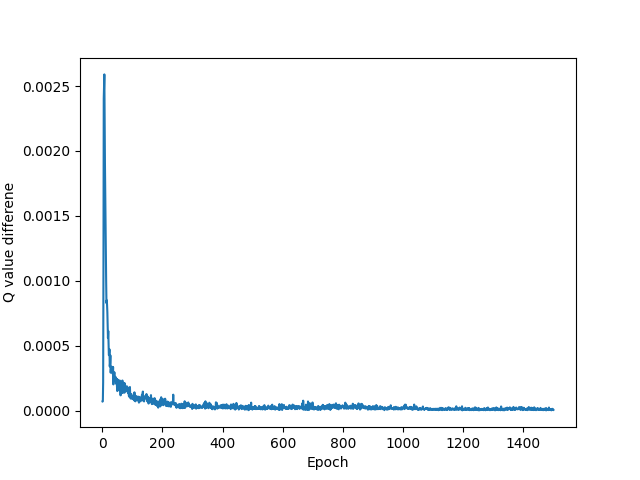
\includegraphics[width=3.6in]{forward.png}	
	\caption{Training curve of the forward module.}
	\label{fig:forward}
\end{figure}


\begin{figure}[!t]
	\centering
	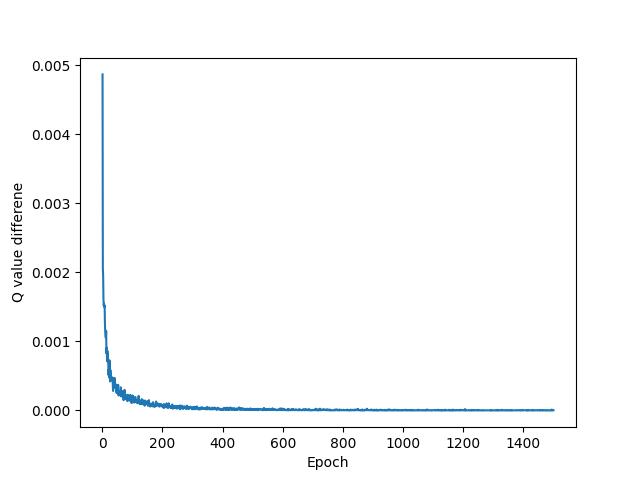
\includegraphics[width=3.6in]{sidewalk.png}	
	\caption{Training curve of the sidewalk module.}
	\label{fig:sidewalk}
\end{figure}

\begin{figure}[!t]
	\centering
	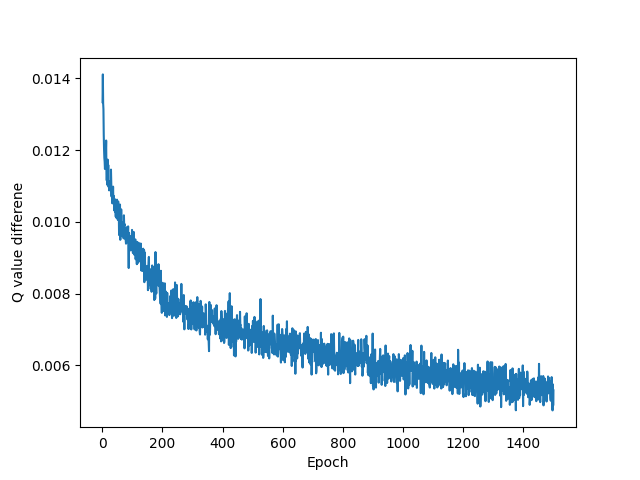
\includegraphics[width=3.6in]{litter.png}	
	\caption{Training curve of the litter module.}
	\label{fig:litter}
\end{figure}


\begin{figure}[!t]
	\centering
	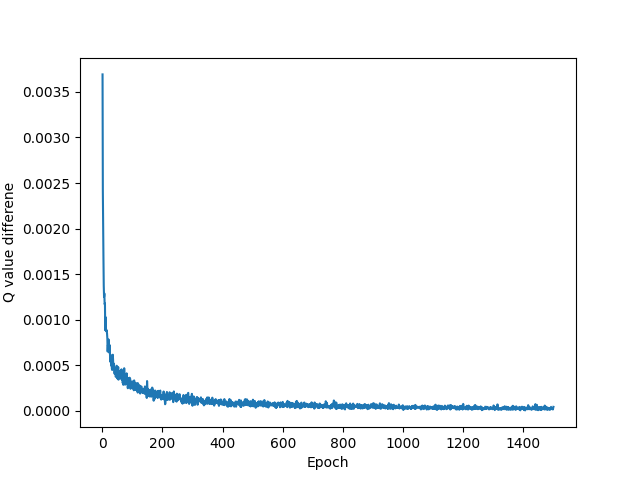
\includegraphics[width=3.6in]{obstacle.png}	
	\caption{Training curve of the obstacle module.}
	\label{fig:obstacle}
\end{figure}


\subsection{Evaluation of each module}
To evaluate each module, we analyze the behavior of each module in the full size grid environment.
Since the sidewalk, litter, obstacle module do not consider the terminal state, weighted sums of one of these module and the forward module were used to evaluate the corresponding module.
The weight used in the combined modules are 0.5 for a target module and 0.5 for the forward module.
The forward module trained to reach terminal state, the forward module was tested independently.
The behavior results of the evaluation are presented in Figure \ref{fig:forward_eval}-\ref{fig:obstacle_eval}.
From the results, it can be concluded that each module was trained to perform the corresponding tasks successfully. 

\subsection{Evaluation of the final module}

To evaluate the final module where all the modules are combined, the module was tested on the full state environment. 
For analysis on the effects of weights $w_i$, we considered two policies.
First, I considered a safe policy that puts more priority on negative rewards from reaching sidewalk and obstacles.
The safe policy uses weights 0.1 for litter and 0.3 for the others.
Second, I considered a greedy policy that puts more priority on positive rewards from collecting litter.
The greedy policy uses weights 0.3 for litter and 0.1 for the others.
The behavior results of these policies are presented in Figure \ref{fig:safe}, \ref{fig:greedy}.
We can find that the greedy policy collected more litter than the safe policy.
From this, we can confirm that the behavior of a policy can be varied depending on the weight setup.
Also, both policies could deal with the multi-purpose tasks, but neither of them performed the optimal trajectory: the safe policy missed one litter grid, and the grid policy collected all the litter with unnecessary trajectory.
This suboptimal issue is caused because each module is trained separately without considering other tasks.
This issue can be solved by using joint optimization while training across different tasks.
 

\section{Summary} %Intermediate/Preliminary Results: State and evaluate your results upeto the milestone

The Q learning algorithm is applied to train an agent to deal with multi-purpose tasks in the assignment. 
To reduce the problem size, single-purpose task modules were trained independently and integrated to deal with multi-purpose tasks.
In addition, by limiting search grids during training, the size of the state space is reduced.
The trained module was evaluated independently and the final module acquired by the weighted sum of each module was tested on the full state environment. 
However, since the full state is not considered in the training environments, the obtained agent does not guarantee global optimality.
Also, the agent shows different behaviors depending on the weights of integrating the task modules.

\begin{figure}[t]
	\centering
	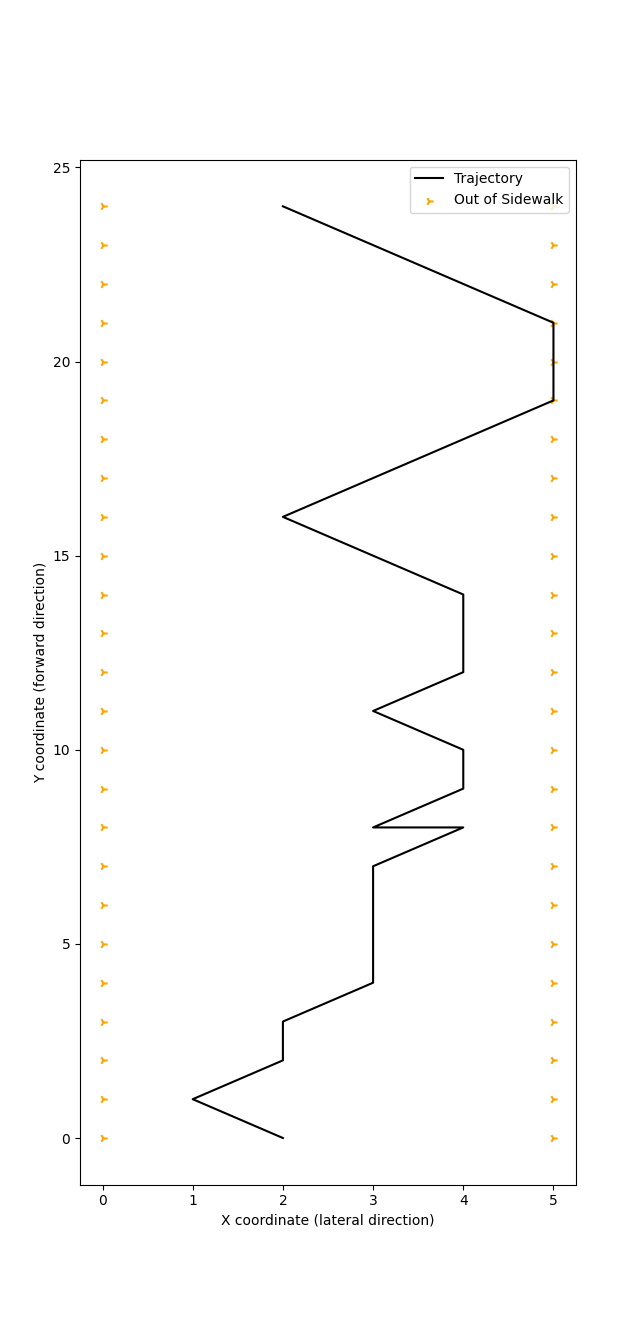
\includegraphics[width=2in]{forward_eval.png}	
	\caption{Behavior of the forward module.}
	\label{fig:forward_eval}
	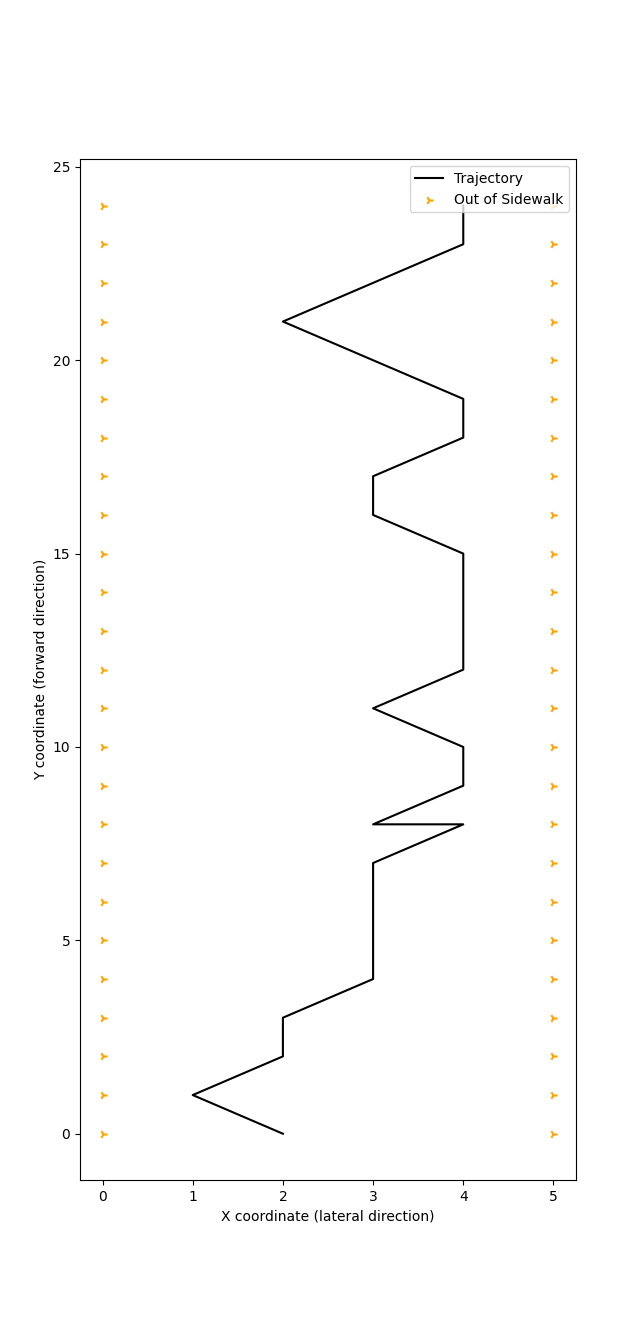
\includegraphics[width=2in]{sidewalk_eval.png}	
	\caption{Behavior of the sidewalk module combined with the forward module.}
	\label{fig:sidewalk_eval}
\end{figure}


\begin{figure}[!t]
	\centering
	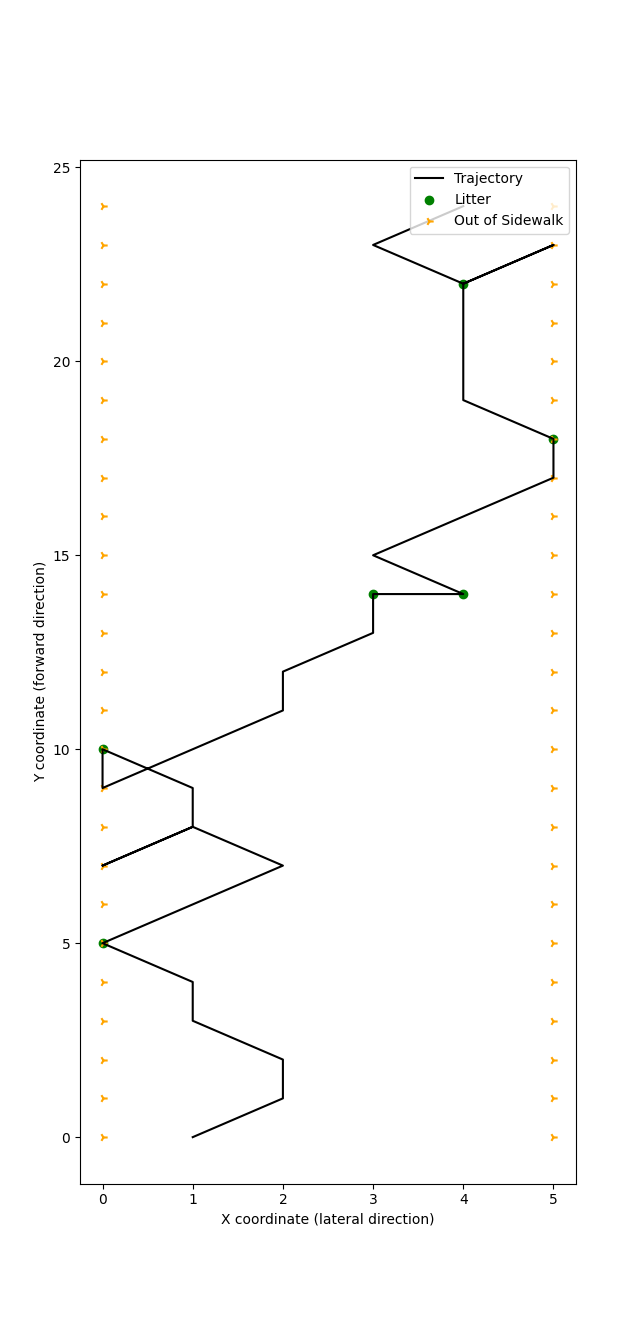
\includegraphics[width=2in]{litter_eval.png}	
	\caption{Behavior of the litter module combined with the forward module.}
	\label{fig:litter_eval}
	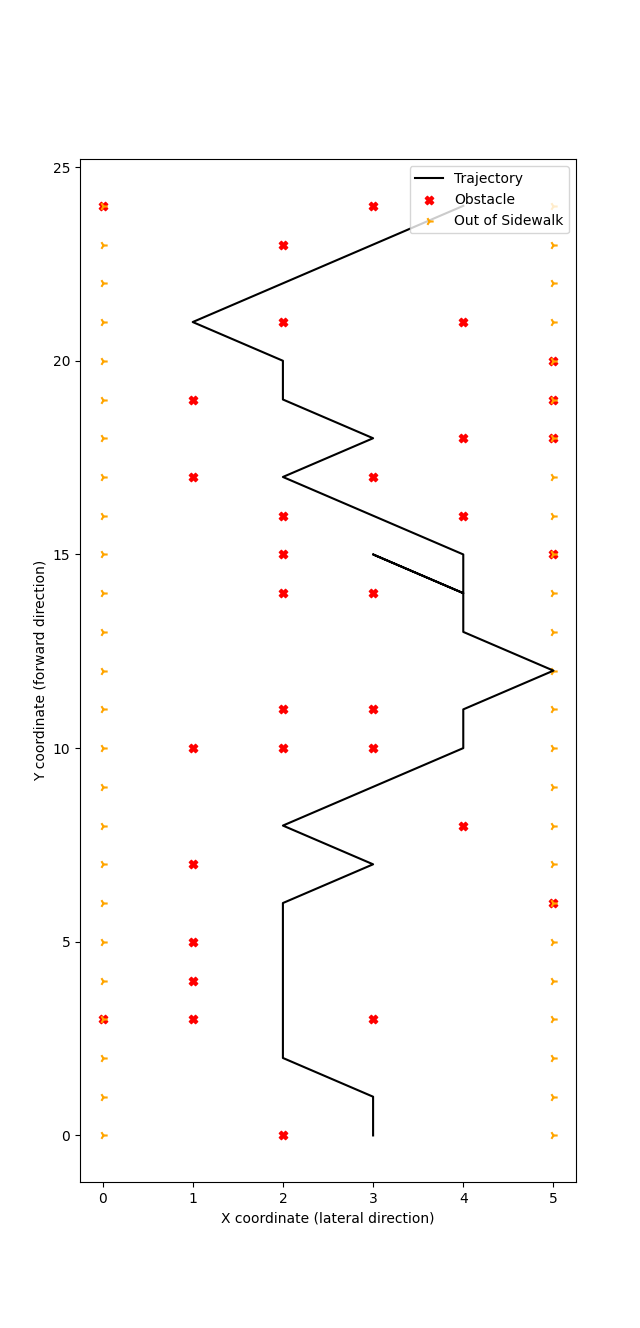
\includegraphics[width=2in]{obstacle_eval.png}	
	\caption{Behavior of the obstacle module combined with the forward module.}
	\label{fig:obstacle_eval}
\end{figure}


\begin{figure}[!t]
	\centering
	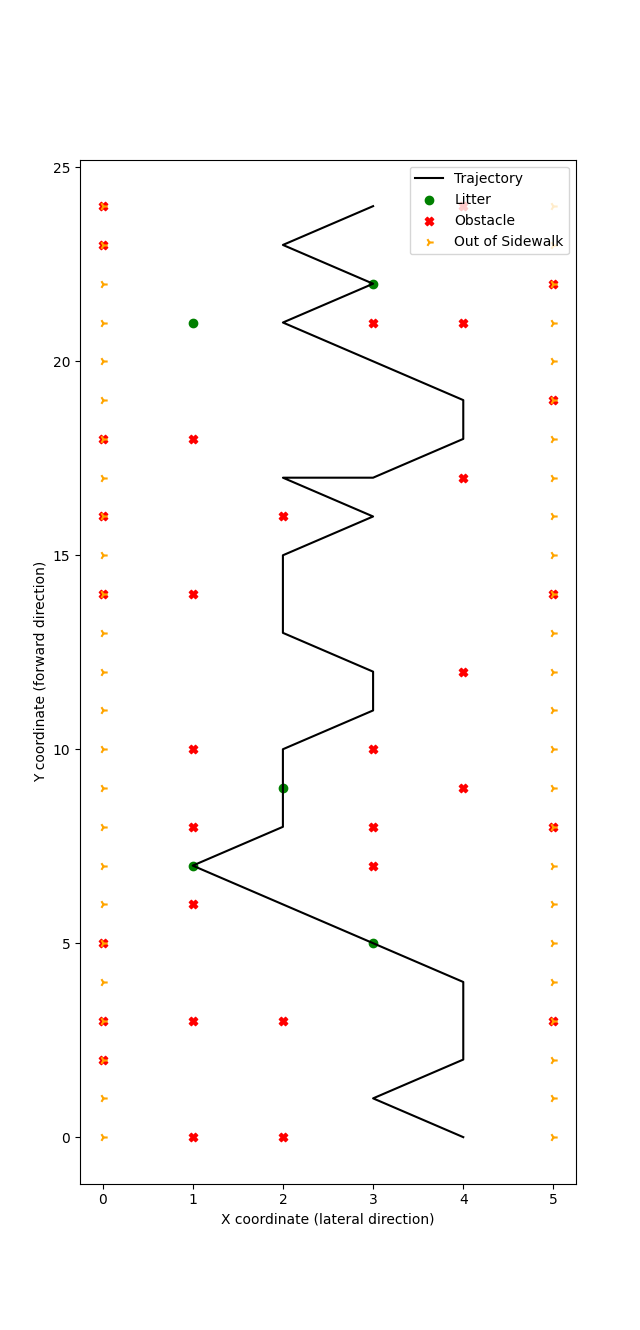
\includegraphics[width=2in]{safe.png}	
	\caption{Behavior of the combined module put more priority on negative rewards.}
	\label{fig:safe}
	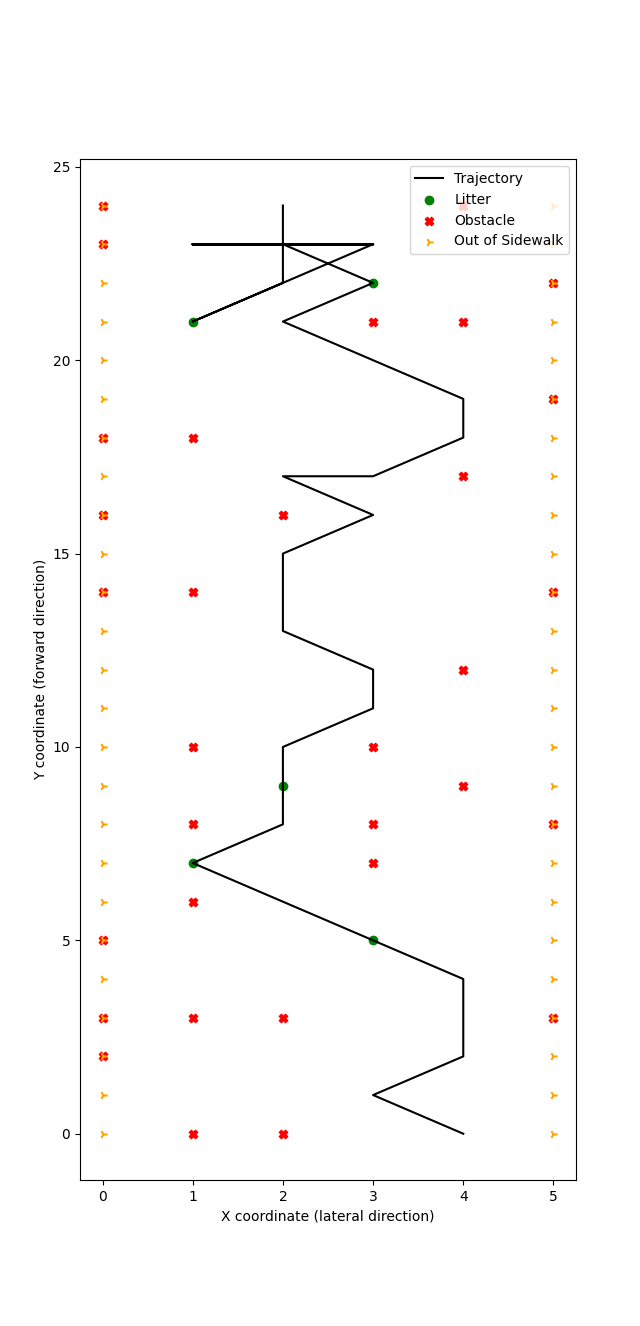
\includegraphics[width=2in]{greedy.png}	
	\caption{Behavior of the combined module put more priority on positive rewards.}
	\label{fig:greedy}
\end{figure}
\end{document}


